\section{目的}
依 Lab 9（PDF 35--38 頁）先調整參考反相器，再比較二輸入 NAND/NOR 的輸入順序、尺寸、轉換曲線、雜訊容限、速度與功率。

\section{Spec 對照}
\begin{longtable}{p{0.31\linewidth}p{0.29\linewidth}p{0.31\linewidth}}
\toprule
講義要求（PDF頁） & 實作 & 驗證與界線 \\\midrule
步驟 1：平衡 INV（35、38） & 01\_inverter\_sizing & 比例 3--7；選 6 \\
步驟 2/3：NAND/NOR 尺寸與 DC（36--38） & 02\_nand、03\_nor、04\_sizing\_refinement & A、B、A=B；完整 NM \\
問題 1/2：最晚輸入、寄生因素（38） & A/B 單獨切換，另一輸入先穩定 & 量兩種輸入位置 \\
問題 3：1.5/2/2.5/3 倍（38） & 02/03 的四個案例 & 比較輸出 rise/fall \\
問題 4：速度、功率、面積（38） & 供應電流平均與寬度和 & 同負載比較；面積僅 proxy \\
\bottomrule
\end{longtable}


\section{電路與設計推導}
固定 $L=0.25\,\mu$m，參考 $W_n=0.6\,\mu$m。先掃 $W_p/W_n=3,4,5,6,7$；選 6 作兩個 gate 的基準。NAND 的 NMOS 串聯、PMOS 並聯；NOR 相反。A 在 NAND 靠輸出端、在 NOR 靠電源端。兩組 gate 各保留 A=B 同時切換、A 切換、B 切換三個條件；NAND 非切換輸入保持 1，NOR 保持 0。

初始串聯寬度乘 K，K=1.5/2/2.5/3，檢查 $R\propto L/W$ 的近似。最後額外調整不同輸入晶體管，改善寄生電容造成的偏差。所選 refinement 第三組：NAND PMOS A/B 寬 4.14/5.04、NMOS 各 1.5；NOR PMOS 各 21.6、NMOS A/B 為 2.7/1.02，單位 $\mu$m。原始 Lab9 第一檔誤接 PWM 外部檔，已以獨立 INV calibration 取代；所有 gate 均自含電路與量測。

\section{模擬設定}
本次為使用另行提供模型的教學改寫，電源為 1.0 V、溫度為 $25\,^{\circ}\mathrm C$。保留講義指定的拓樸、負載及比較尺寸；原講義的 2.5 V 製程結果不是本次模型的驗收數值。1 V 僅是模擬條件，不能視為模型的安全額定。所有 MOS 的 Bulk 明確接至相應電源軌。

HSPICE S-2021.09 使用 RUNLVL=6；保存波形、列印資料及原生量測。圖表由本次數據重繪；CSV 保存於各 Lab 的 results。完成模擬表示求解成功，並不代表製程可靠度已驗證。加密模型仍有被抑制的警告；既有診斷未取得可判讀的進一步內容，因此不宣稱警告無害或全部模型限制已滿足。

所有輸出接 20 fF，輸入邊緣 0.1 ns、週期 5 ns、模擬 15 ns、列印 1 ps。DC 0--1 V、0.5 mV。供應功率在 5--15 ns 的完整週期平均，為電源端功率，不含理想輸入訊號源能量。NM 採 Lab8 的邊界輸出定義。講義只要求「大約相等」而未給容差；本文另以 10\% 作尺寸調整的工程比較目標，並非原講義通過門檻。

\section{結果與規格檢查}
四份 deck、16 個案例皆完成且無失敗量測。
\begin{center}\small
\begin{tabular}{llll}
\toprule
$W_p/W_n$ & $V_M$ (V) & $t_r$ (ps) & $t_f$ (ps) \\
\midrule
3 & 0.4825 & 222.64 & 110.85 \\
4 & 0.4956 & 173.83 & 113.49 \\
5 & 0.5058 & 144.13 & 115.26 \\
6 & 0.5142 & 124.85 & 117.32 \\
7 & 0.5212 & 110.93 & 119.71 \\
\bottomrule
\end{tabular}
\end{center}
\begin{center}\small
\begin{tabular}{lllll}
\toprule
Gate & Input & $V_M$ (V) & $NM_L$ (V) & $NM_H$ (V) \\
\midrule
NAND & both & 0.5464 & 0.4615 & 0.3621 \\
NAND & a & 0.4923 & 0.3924 & 0.4226 \\
NAND & b & 0.4827 & 0.3808 & 0.4331 \\
NOR & both & 0.4792 & 0.3849 & 0.4430 \\
NOR & a & 0.5455 & 0.4539 & 0.3585 \\
NOR & b & 0.5352 & 0.4442 & 0.3712 \\
\bottomrule
\end{tabular}
\end{center}

\begin{figure}[htbp]
\centering
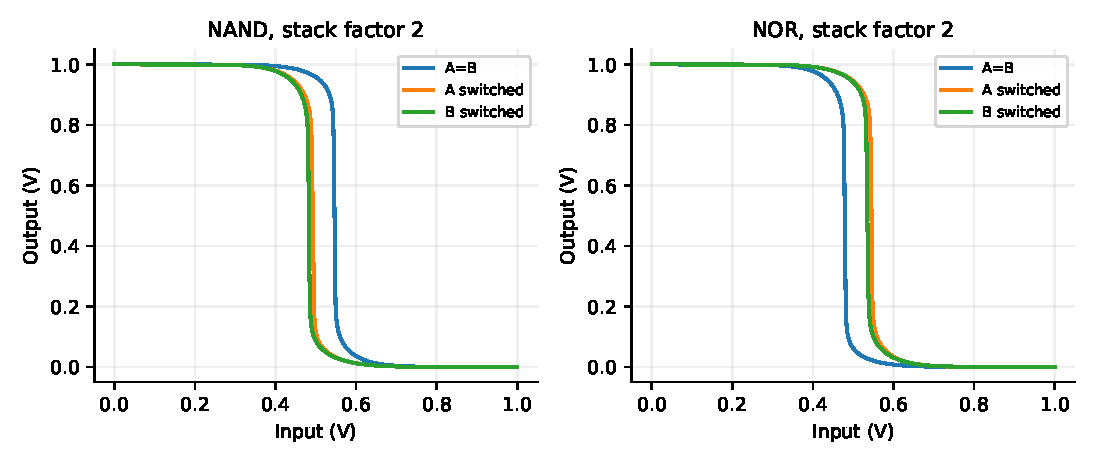
\includegraphics[width=\linewidth]{figures/gate_transfer.pdf}
\caption{串聯倍率 2 的三種輸入 VTC；由本次 HSPICE 數據重繪。}
\end{figure}
\begin{center}\small
\begin{tabular}{lllll}
\toprule
Selected design & $t_r$ (ps) & $t_f$ (ps) & $t_{pHL}$ (ps) & $t_{pLH}$ (ps) \\
\midrule
INV & 123.30 & 116.03 & 109.74 & 96.30 \\
NAND A & 130.26 & 111.14 & 99.02 & 102.50 \\
NAND B & 124.24 & 111.18 & 107.10 & 104.32 \\
NOR A & 134.89 & 122.00 & 135.99 & 121.49 \\
NOR B & 128.66 & 116.35 & 150.46 & 79.97 \\
\bottomrule
\end{tabular}
\end{center}

\begin{figure}[htbp]
\centering
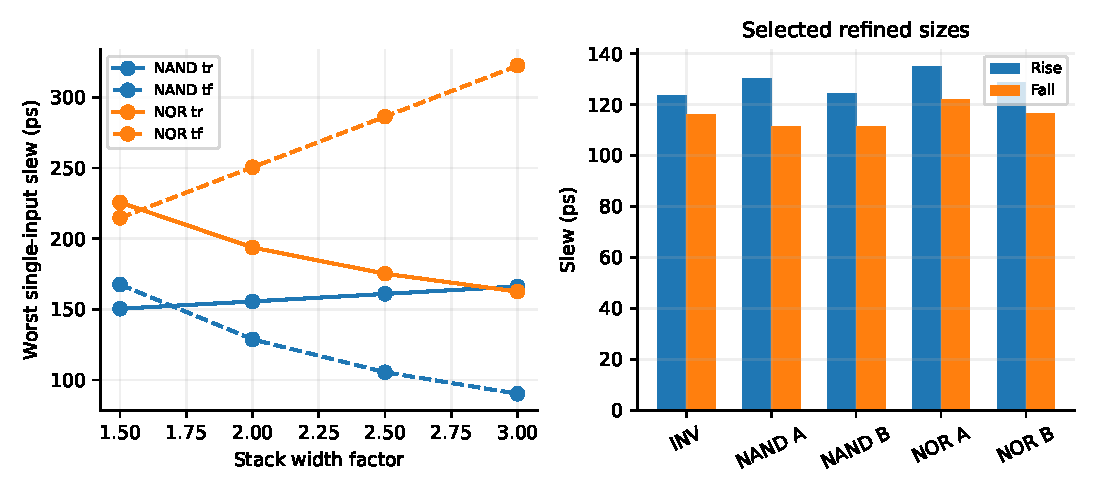
\includegraphics[width=\linewidth]{figures/gate_sizing.pdf}
\caption{倍率比較與最後尺寸調整；由本次 HSPICE 數據重繪。}
\end{figure}
初始 K=2 的平均供應功率與寬度總和：
\begin{center}\small
\begin{tabular}{lllll}
\toprule
Gate & $P_{A=B}$ ($\mu$W) & $P_A$ ($\mu$W) & $P_B$ ($\mu$W) & $\sum W$ ($\mu$m) \\
\midrule
NAND & 7.145 & 6.480 & 7.299 & 9.6 \\
NOR & 9.134 & 12.916 & 7.232 & 15.6 \\
\bottomrule
\end{tabular}
\end{center}


\section{討論}
比例 6 的 INV 門檻約 0.514 V，rise/fall 約 124.85/117.32 ps，已接近但不完全對稱。最後 refinement 的四種單輸入 slew 相對同 deck 參考最大偏差約 9.4\%；同時切換兩個並聯管會較快，不能要求所有輸入模式均有相同延遲。

最晚到的訊號宜接串聯網路靠輸出端的 MOS：NAND 為 A、NOR 為 B。本測試讓另一輸入預先穩定，直接比較這個條件；內部節點必須充放電及 body effect 使單純串聯數倍寬度不是精確法則。加寬也增加接面／重疊電容及輸入負載。初始 K=2 的寬度總和 NAND 為 9.6、NOR 為 15.6 $\mu$m；這只是相同 L 下的有源寬度 proxy，未包含布局、接點與布線。各輸入模式的平均供應功率保存在 CSV；NOR 在本次等負載比較通常較慢且耗能較高，但面積／功耗沒有跨製程的絕對排名。為取得 slew 接近而大幅加寬 NOR 會增加面積與輸入負載，並非免費改善。

\section{結論}
三步驟與四個問題均有相對應測試；先保留講義倍率，再補尺寸改善。所列約 10\% matching 是本次工程目標的結果，原製程數據與未知可靠度限制仍未宣稱滿足。
